% Created by tikzDevice version 0.7.0 on 2014-07-24 03:38:08
% !TEX encoding = UTF-8 Unicode
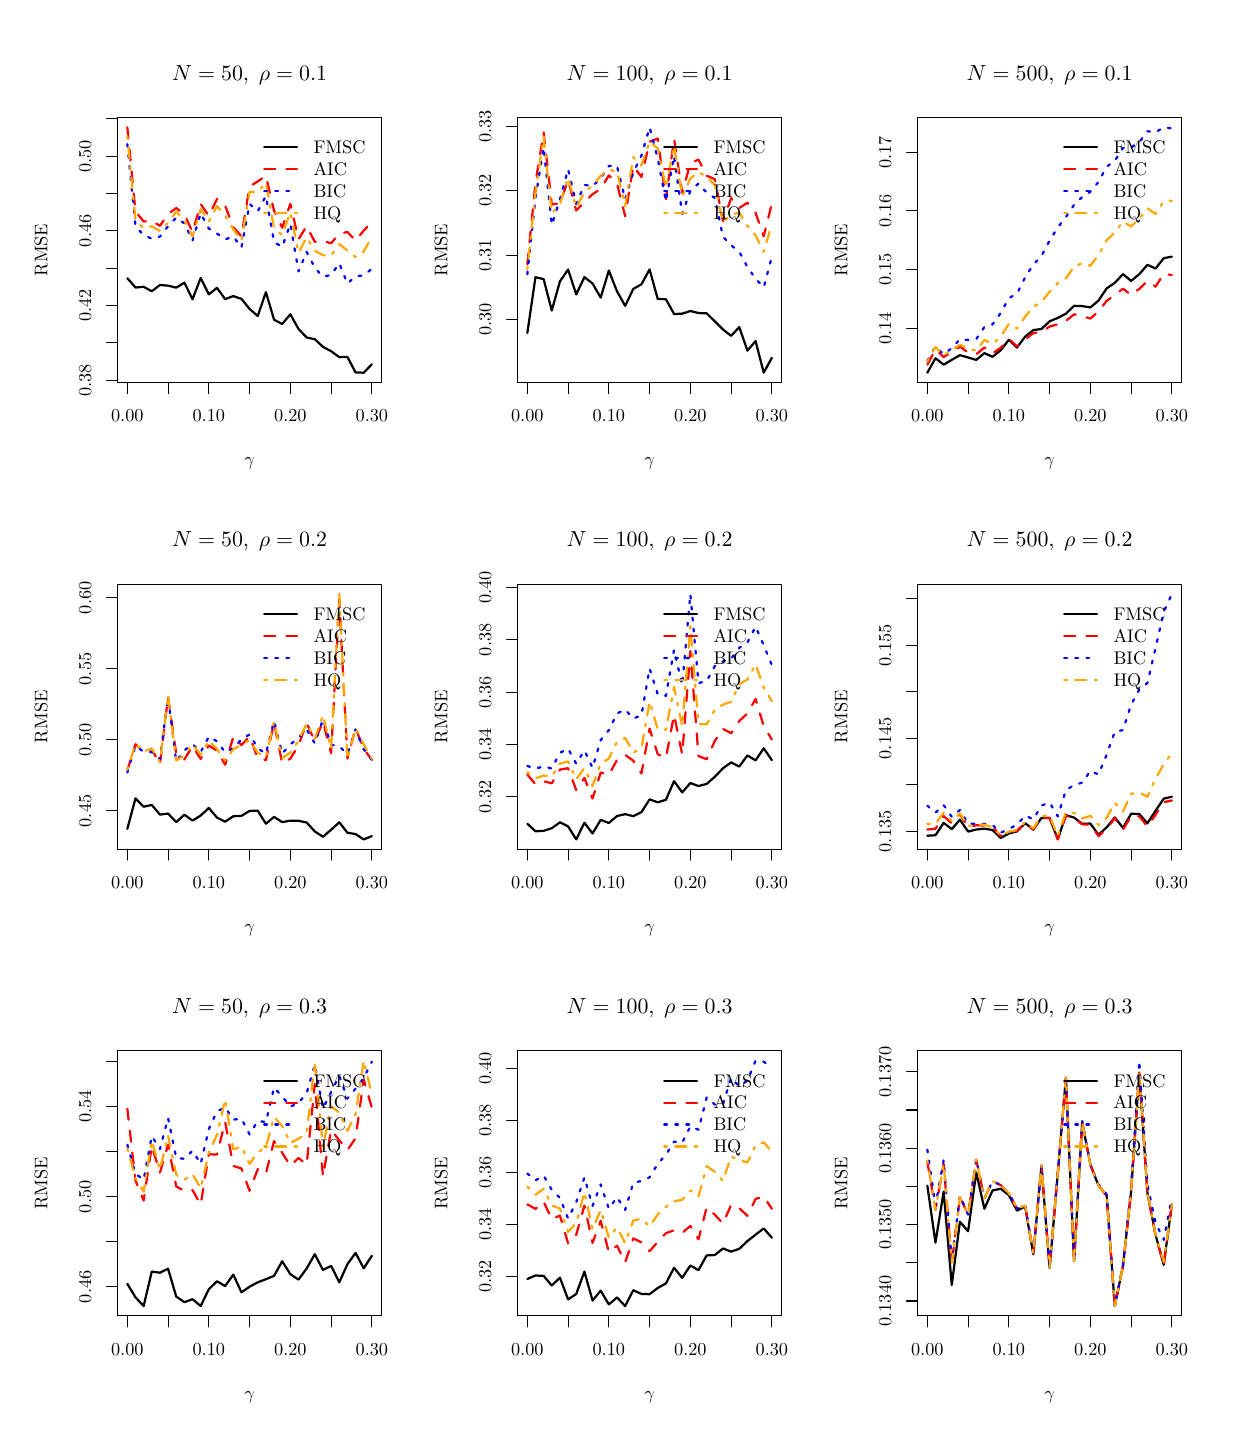
\begin{tikzpicture}[x=1pt,y=1pt]
\definecolor[named]{fillColor}{rgb}{1.00,1.00,1.00}
\path[use as bounding box,fill=fillColor,fill opacity=0.00] (0,0) rectangle (433.62,505.89);
\begin{scope}
\path[clip] ( 32.47,377.65) rectangle (127.91,473.42);
\definecolor[named]{drawColor}{rgb}{0.00,0.00,0.00}

\path[draw=drawColor,line width= 0.8pt,line join=round,line cap=round] ( 36.01,415.37) --
	( 38.95,411.99) --
	( 41.90,412.26) --
	( 44.84,410.63) --
	( 47.79,412.90) --
	( 50.73,412.66) --
	( 53.68,411.95) --
	( 56.63,413.73) --
	( 59.57,407.76) --
	( 62.52,415.43) --
	( 65.46,409.51) --
	( 68.41,411.87) --
	( 71.35,407.78) --
	( 74.30,408.89) --
	( 77.24,407.90) --
	( 80.19,404.23) --
	( 83.14,401.68) --
	( 86.08,410.33) --
	( 89.03,400.37) --
	( 91.97,398.80) --
	( 94.92,402.33) --
	( 97.86,397.04) --
	(100.81,393.93) --
	(103.75,393.31) --
	(106.70,390.55) --
	(109.65,388.98) --
	(112.59,386.83) --
	(115.54,386.89) --
	(118.48,381.32) --
	(121.43,381.20) --
	(124.37,384.25);
\end{scope}
\begin{scope}
\path[clip] (  0.00,  0.00) rectangle (433.62,505.89);
\definecolor[named]{drawColor}{rgb}{0.00,0.00,0.00}

\path[draw=drawColor,line width= 0.4pt,line join=round,line cap=round] ( 36.01,377.65) -- (124.37,377.65);

\path[draw=drawColor,line width= 0.4pt,line join=round,line cap=round] ( 36.01,377.65) -- ( 36.01,373.69);

\path[draw=drawColor,line width= 0.4pt,line join=round,line cap=round] ( 50.73,377.65) -- ( 50.73,373.69);

\path[draw=drawColor,line width= 0.4pt,line join=round,line cap=round] ( 65.46,377.65) -- ( 65.46,373.69);

\path[draw=drawColor,line width= 0.4pt,line join=round,line cap=round] ( 80.19,377.65) -- ( 80.19,373.69);

\path[draw=drawColor,line width= 0.4pt,line join=round,line cap=round] ( 94.92,377.65) -- ( 94.92,373.69);

\path[draw=drawColor,line width= 0.4pt,line join=round,line cap=round] (109.65,377.65) -- (109.65,373.69);

\path[draw=drawColor,line width= 0.4pt,line join=round,line cap=round] (124.37,377.65) -- (124.37,373.69);

\node[text=drawColor,anchor=base,inner sep=0pt, outer sep=0pt, scale=  0.66] at ( 36.01,363.40) {0.00};

\node[text=drawColor,anchor=base,inner sep=0pt, outer sep=0pt, scale=  0.66] at ( 65.46,363.40) {0.10};

\node[text=drawColor,anchor=base,inner sep=0pt, outer sep=0pt, scale=  0.66] at ( 94.92,363.40) {0.20};

\node[text=drawColor,anchor=base,inner sep=0pt, outer sep=0pt, scale=  0.66] at (124.37,363.40) {0.30};

\path[draw=drawColor,line width= 0.4pt,line join=round,line cap=round] ( 32.47,378.52) -- ( 32.47,472.91);

\path[draw=drawColor,line width= 0.4pt,line join=round,line cap=round] ( 32.47,378.52) -- ( 28.51,378.52);

\path[draw=drawColor,line width= 0.4pt,line join=round,line cap=round] ( 32.47,392.00) -- ( 28.51,392.00);

\path[draw=drawColor,line width= 0.4pt,line join=round,line cap=round] ( 32.47,405.49) -- ( 28.51,405.49);

\path[draw=drawColor,line width= 0.4pt,line join=round,line cap=round] ( 32.47,418.97) -- ( 28.51,418.97);

\path[draw=drawColor,line width= 0.4pt,line join=round,line cap=round] ( 32.47,432.46) -- ( 28.51,432.46);

\path[draw=drawColor,line width= 0.4pt,line join=round,line cap=round] ( 32.47,445.94) -- ( 28.51,445.94);

\path[draw=drawColor,line width= 0.4pt,line join=round,line cap=round] ( 32.47,459.42) -- ( 28.51,459.42);

\path[draw=drawColor,line width= 0.4pt,line join=round,line cap=round] ( 32.47,472.91) -- ( 28.51,472.91);

\node[text=drawColor,rotate= 90.00,anchor=base,inner sep=0pt, outer sep=0pt, scale=  0.66] at ( 22.97,378.52) {0.38};

\node[text=drawColor,rotate= 90.00,anchor=base,inner sep=0pt, outer sep=0pt, scale=  0.66] at ( 22.97,405.49) {0.42};

\node[text=drawColor,rotate= 90.00,anchor=base,inner sep=0pt, outer sep=0pt, scale=  0.66] at ( 22.97,432.46) {0.46};

\node[text=drawColor,rotate= 90.00,anchor=base,inner sep=0pt, outer sep=0pt, scale=  0.66] at ( 22.97,459.42) {0.50};

\path[draw=drawColor,line width= 0.4pt,line join=round,line cap=round] ( 32.47,377.65) --
	(127.91,377.65) --
	(127.91,473.42) --
	( 32.47,473.42) --
	( 32.47,377.65);
\end{scope}
\begin{scope}
\path[clip] (  0.00,337.26) rectangle (144.54,505.89);
\definecolor[named]{drawColor}{rgb}{0.00,0.00,0.00}

\node[text=drawColor,anchor=base,inner sep=0pt, outer sep=0pt, scale=  0.79] at ( 80.19,486.92) {\bfseries $N=50, \;\rho=0.1$};

\node[text=drawColor,anchor=base,inner sep=0pt, outer sep=0pt, scale=  0.66] at ( 80.19,347.56) {$\gamma$};

\node[text=drawColor,rotate= 90.00,anchor=base,inner sep=0pt, outer sep=0pt, scale=  0.66] at (  7.13,425.53) {RMSE};
\end{scope}
\begin{scope}
\path[clip] ( 32.47,377.65) rectangle (127.91,473.42);
\definecolor[named]{drawColor}{rgb}{1.00,0.00,0.00}

\path[draw=drawColor,line width= 0.8pt,dash pattern=on 4pt off 4pt ,line join=round,line cap=round] ( 36.01,469.87) --
	( 38.95,439.52) --
	( 41.90,435.85) --
	( 44.84,436.11) --
	( 47.79,434.27) --
	( 50.73,438.59) --
	( 53.68,440.68) --
	( 56.63,438.48) --
	( 59.57,432.03) --
	( 62.52,442.17) --
	( 65.46,437.84) --
	( 68.41,443.99) --
	( 71.35,441.53) --
	( 74.30,433.79) --
	( 77.24,430.47) --
	( 80.19,448.54) --
	( 83.14,450.33) --
	( 86.08,452.34) --
	( 89.03,439.67) --
	( 91.97,433.62) --
	( 94.92,442.23) --
	( 97.86,429.44) --
	(100.81,434.16) --
	(103.75,428.49) --
	(106.70,428.83) --
	(109.65,427.99) --
	(112.59,431.42) --
	(115.54,432.06) --
	(118.48,428.97) --
	(121.43,432.55) --
	(124.37,435.65);
\definecolor[named]{drawColor}{rgb}{0.00,0.00,1.00}

\path[draw=drawColor,line width= 0.8pt,dash pattern=on 1pt off 3pt ,line join=round,line cap=round] ( 36.01,463.83) --
	( 38.95,434.16) --
	( 41.90,430.90) --
	( 44.84,429.65) --
	( 47.79,430.40) --
	( 50.73,434.12) --
	( 53.68,437.24) --
	( 56.63,435.16) --
	( 59.57,428.96) --
	( 62.52,438.82) --
	( 65.46,433.31) --
	( 68.41,431.50) --
	( 71.35,429.37) --
	( 74.30,430.42) --
	( 77.24,426.43) --
	( 80.19,442.21) --
	( 83.14,439.55) --
	( 86.08,445.07) --
	( 89.03,428.42) --
	( 91.97,426.68) --
	( 94.92,434.96) --
	( 97.86,417.82) --
	(100.81,424.85) --
	(103.75,419.16) --
	(106.70,415.84) --
	(109.65,416.56) --
	(112.59,420.74) --
	(115.54,413.42) --
	(118.48,416.03) --
	(121.43,416.39) --
	(124.37,418.75);
\definecolor[named]{drawColor}{rgb}{1.00,0.65,0.00}

\path[draw=drawColor,line width= 0.8pt,dash pattern=on 1pt off 3pt on 4pt off 3pt ,line join=round,line cap=round] ( 36.01,466.72) --
	( 38.95,436.33) --
	( 41.90,433.44) --
	( 44.84,434.10) --
	( 47.79,432.42) --
	( 50.73,435.35) --
	( 53.68,439.42) --
	( 56.63,436.15) --
	( 59.57,430.35) --
	( 62.52,440.30) --
	( 65.46,435.82) --
	( 68.41,441.42) --
	( 71.35,437.98) --
	( 74.30,433.08) --
	( 77.24,428.97) --
	( 80.19,446.59) --
	( 83.14,446.46) --
	( 86.08,449.86) --
	( 89.03,433.30) --
	( 91.97,431.04) --
	( 94.92,439.15) --
	( 97.86,424.51) --
	(100.81,430.13) --
	(103.75,425.25) --
	(106.70,423.66) --
	(109.65,423.57) --
	(112.59,427.72) --
	(115.54,425.34) --
	(118.48,423.06) --
	(121.43,425.01) --
	(124.37,430.37);
\definecolor[named]{drawColor}{rgb}{0.00,0.00,0.00}

\path[draw=drawColor,line width= 0.8pt,line join=round,line cap=round] ( 85.47,462.63) -- ( 97.35,462.63);
\definecolor[named]{drawColor}{rgb}{1.00,0.00,0.00}

\path[draw=drawColor,line width= 0.8pt,dash pattern=on 4pt off 4pt ,line join=round,line cap=round] ( 85.47,454.71) -- ( 97.35,454.71);
\definecolor[named]{drawColor}{rgb}{0.00,0.00,1.00}

\path[draw=drawColor,line width= 0.8pt,dash pattern=on 1pt off 3pt ,line join=round,line cap=round] ( 85.47,446.79) -- ( 97.35,446.79);
\definecolor[named]{drawColor}{rgb}{1.00,0.65,0.00}

\path[draw=drawColor,line width= 0.8pt,dash pattern=on 1pt off 3pt on 4pt off 3pt ,line join=round,line cap=round] ( 85.47,438.87) -- ( 97.35,438.87);
\definecolor[named]{drawColor}{rgb}{0.00,0.00,0.00}

\node[text=drawColor,anchor=base west,inner sep=0pt, outer sep=0pt, scale=  0.66] at (103.29,460.35) {FMSC};

\node[text=drawColor,anchor=base west,inner sep=0pt, outer sep=0pt, scale=  0.66] at (103.29,452.43) {AIC};

\node[text=drawColor,anchor=base west,inner sep=0pt, outer sep=0pt, scale=  0.66] at (103.29,444.51) {BIC};

\node[text=drawColor,anchor=base west,inner sep=0pt, outer sep=0pt, scale=  0.66] at (103.29,436.59) {HQ};
\end{scope}
\begin{scope}
\path[clip] (177.01,377.65) rectangle (272.45,473.42);
\definecolor[named]{drawColor}{rgb}{0.00,0.00,0.00}

\path[draw=drawColor,line width= 0.8pt,line join=round,line cap=round] (180.55,395.55) --
	(183.49,415.74) --
	(186.44,415.01) --
	(189.38,403.66) --
	(192.33,414.22) --
	(195.27,418.48) --
	(198.22,409.50) --
	(201.17,415.74) --
	(204.11,413.45) --
	(207.06,408.35) --
	(210.00,418.14) --
	(212.95,410.63) --
	(215.89,405.36) --
	(218.84,411.48) --
	(221.78,413.16) --
	(224.73,418.52) --
	(227.68,407.82) --
	(230.62,407.78) --
	(233.57,402.42) --
	(236.51,402.54) --
	(239.46,403.49) --
	(242.40,402.77) --
	(245.35,402.66) --
	(248.29,399.77) --
	(251.24,396.82) --
	(254.19,394.54) --
	(257.13,397.69) --
	(260.08,389.17) --
	(263.02,392.64) --
	(265.97,381.20) --
	(268.91,386.61);
\end{scope}
\begin{scope}
\path[clip] (  0.00,  0.00) rectangle (433.62,505.89);
\definecolor[named]{drawColor}{rgb}{0.00,0.00,0.00}

\path[draw=drawColor,line width= 0.4pt,line join=round,line cap=round] (180.55,377.65) -- (268.91,377.65);

\path[draw=drawColor,line width= 0.4pt,line join=round,line cap=round] (180.55,377.65) -- (180.55,373.69);

\path[draw=drawColor,line width= 0.4pt,line join=round,line cap=round] (195.27,377.65) -- (195.27,373.69);

\path[draw=drawColor,line width= 0.4pt,line join=round,line cap=round] (210.00,377.65) -- (210.00,373.69);

\path[draw=drawColor,line width= 0.4pt,line join=round,line cap=round] (224.73,377.65) -- (224.73,373.69);

\path[draw=drawColor,line width= 0.4pt,line join=round,line cap=round] (239.46,377.65) -- (239.46,373.69);

\path[draw=drawColor,line width= 0.4pt,line join=round,line cap=round] (254.19,377.65) -- (254.19,373.69);

\path[draw=drawColor,line width= 0.4pt,line join=round,line cap=round] (268.91,377.65) -- (268.91,373.69);

\node[text=drawColor,anchor=base,inner sep=0pt, outer sep=0pt, scale=  0.66] at (180.55,363.40) {0.00};

\node[text=drawColor,anchor=base,inner sep=0pt, outer sep=0pt, scale=  0.66] at (210.00,363.40) {0.10};

\node[text=drawColor,anchor=base,inner sep=0pt, outer sep=0pt, scale=  0.66] at (239.46,363.40) {0.20};

\node[text=drawColor,anchor=base,inner sep=0pt, outer sep=0pt, scale=  0.66] at (268.91,363.40) {0.30};

\path[draw=drawColor,line width= 0.4pt,line join=round,line cap=round] (177.01,400.44) -- (177.01,470.23);

\path[draw=drawColor,line width= 0.4pt,line join=round,line cap=round] (177.01,400.44) -- (173.05,400.44);

\path[draw=drawColor,line width= 0.4pt,line join=round,line cap=round] (177.01,423.70) -- (173.05,423.70);

\path[draw=drawColor,line width= 0.4pt,line join=round,line cap=round] (177.01,446.97) -- (173.05,446.97);

\path[draw=drawColor,line width= 0.4pt,line join=round,line cap=round] (177.01,470.23) -- (173.05,470.23);

\node[text=drawColor,rotate= 90.00,anchor=base,inner sep=0pt, outer sep=0pt, scale=  0.66] at (167.51,400.44) {0.30};

\node[text=drawColor,rotate= 90.00,anchor=base,inner sep=0pt, outer sep=0pt, scale=  0.66] at (167.51,423.70) {0.31};

\node[text=drawColor,rotate= 90.00,anchor=base,inner sep=0pt, outer sep=0pt, scale=  0.66] at (167.51,446.97) {0.32};

\node[text=drawColor,rotate= 90.00,anchor=base,inner sep=0pt, outer sep=0pt, scale=  0.66] at (167.51,470.23) {0.33};

\path[draw=drawColor,line width= 0.4pt,line join=round,line cap=round] (177.01,377.65) --
	(272.45,377.65) --
	(272.45,473.42) --
	(177.01,473.42) --
	(177.01,377.65);
\end{scope}
\begin{scope}
\path[clip] (144.54,337.26) rectangle (289.08,505.89);
\definecolor[named]{drawColor}{rgb}{0.00,0.00,0.00}

\node[text=drawColor,anchor=base,inner sep=0pt, outer sep=0pt, scale=  0.79] at (224.73,486.92) {\bfseries $N=100, \;\rho=0.1$};

\node[text=drawColor,anchor=base,inner sep=0pt, outer sep=0pt, scale=  0.66] at (224.73,347.56) {$\gamma$};

\node[text=drawColor,rotate= 90.00,anchor=base,inner sep=0pt, outer sep=0pt, scale=  0.66] at (151.67,425.53) {RMSE};
\end{scope}
\begin{scope}
\path[clip] (177.01,377.65) rectangle (272.45,473.42);
\definecolor[named]{drawColor}{rgb}{1.00,0.00,0.00}

\path[draw=drawColor,line width= 0.8pt,dash pattern=on 4pt off 4pt ,line join=round,line cap=round] (180.55,420.40) --
	(183.49,449.76) --
	(186.44,468.01) --
	(189.38,442.06) --
	(192.33,442.37) --
	(195.27,450.85) --
	(198.22,439.84) --
	(201.17,442.88) --
	(204.11,445.72) --
	(207.06,447.58) --
	(210.00,452.51) --
	(212.95,449.54) --
	(215.89,437.75) --
	(218.84,455.96) --
	(221.78,451.92) --
	(224.73,464.67) --
	(227.68,465.84) --
	(230.62,443.91) --
	(233.57,465.79) --
	(236.51,446.17) --
	(239.46,456.91) --
	(242.40,458.23) --
	(245.35,452.40) --
	(248.29,451.12) --
	(251.24,436.03) --
	(254.19,444.26) --
	(257.13,440.70) --
	(260.08,442.65) --
	(263.02,438.99) --
	(265.97,430.53) --
	(268.91,442.34);
\definecolor[named]{drawColor}{rgb}{0.00,0.00,1.00}

\path[draw=drawColor,line width= 0.8pt,dash pattern=on 1pt off 3pt ,line join=round,line cap=round] (180.55,416.77) --
	(183.49,444.26) --
	(186.44,462.60) --
	(189.38,434.62) --
	(192.33,443.85) --
	(195.27,454.74) --
	(198.22,442.17) --
	(201.17,449.12) --
	(204.11,448.56) --
	(207.06,451.44) --
	(210.00,455.92) --
	(212.95,455.94) --
	(215.89,443.87) --
	(218.84,453.60) --
	(221.78,459.67) --
	(224.73,469.87) --
	(227.68,458.60) --
	(230.62,443.18) --
	(233.57,459.53) --
	(236.51,438.59) --
	(239.46,446.95) --
	(242.40,449.57) --
	(245.35,446.26) --
	(248.29,444.36) --
	(251.24,430.37) --
	(254.19,427.26) --
	(257.13,424.93) --
	(260.08,419.41) --
	(263.02,415.18) --
	(265.97,412.03) --
	(268.91,423.17);
\definecolor[named]{drawColor}{rgb}{1.00,0.65,0.00}

\path[draw=drawColor,line width= 0.8pt,dash pattern=on 1pt off 3pt on 4pt off 3pt ,line join=round,line cap=round] (180.55,418.57) --
	(183.49,446.19) --
	(186.44,466.47) --
	(189.38,438.79) --
	(192.33,442.01) --
	(195.27,451.72) --
	(198.22,440.87) --
	(201.17,446.45) --
	(204.11,448.89) --
	(207.06,452.36) --
	(210.00,454.52) --
	(212.95,453.94) --
	(215.89,441.32) --
	(218.84,459.10) --
	(221.78,456.11) --
	(224.73,464.68) --
	(227.68,462.24) --
	(230.62,448.15) --
	(233.57,463.18) --
	(236.51,445.01) --
	(239.46,451.40) --
	(242.40,453.71) --
	(245.35,452.01) --
	(248.29,448.97) --
	(251.24,435.47) --
	(254.19,438.37) --
	(257.13,438.99) --
	(260.08,434.26) --
	(263.02,430.83) --
	(265.97,424.91) --
	(268.91,434.88);
\definecolor[named]{drawColor}{rgb}{0.00,0.00,0.00}

\path[draw=drawColor,line width= 0.8pt,line join=round,line cap=round] (230.01,462.63) -- (241.89,462.63);
\definecolor[named]{drawColor}{rgb}{1.00,0.00,0.00}

\path[draw=drawColor,line width= 0.8pt,dash pattern=on 4pt off 4pt ,line join=round,line cap=round] (230.01,454.71) -- (241.89,454.71);
\definecolor[named]{drawColor}{rgb}{0.00,0.00,1.00}

\path[draw=drawColor,line width= 0.8pt,dash pattern=on 1pt off 3pt ,line join=round,line cap=round] (230.01,446.79) -- (241.89,446.79);
\definecolor[named]{drawColor}{rgb}{1.00,0.65,0.00}

\path[draw=drawColor,line width= 0.8pt,dash pattern=on 1pt off 3pt on 4pt off 3pt ,line join=round,line cap=round] (230.01,438.87) -- (241.89,438.87);
\definecolor[named]{drawColor}{rgb}{0.00,0.00,0.00}

\node[text=drawColor,anchor=base west,inner sep=0pt, outer sep=0pt, scale=  0.66] at (247.83,460.35) {FMSC};

\node[text=drawColor,anchor=base west,inner sep=0pt, outer sep=0pt, scale=  0.66] at (247.83,452.43) {AIC};

\node[text=drawColor,anchor=base west,inner sep=0pt, outer sep=0pt, scale=  0.66] at (247.83,444.51) {BIC};

\node[text=drawColor,anchor=base west,inner sep=0pt, outer sep=0pt, scale=  0.66] at (247.83,436.59) {HQ};
\end{scope}
\begin{scope}
\path[clip] (321.55,377.65) rectangle (416.99,473.42);
\definecolor[named]{drawColor}{rgb}{0.00,0.00,0.00}

\path[draw=drawColor,line width= 0.8pt,line join=round,line cap=round] (325.09,381.20) --
	(328.03,386.44) --
	(330.98,384.11) --
	(333.92,385.87) --
	(336.87,387.54) --
	(339.81,386.71) --
	(342.76,385.84) --
	(345.71,388.27) --
	(348.65,386.96) --
	(351.60,389.32) --
	(354.54,393.10) --
	(357.49,390.32) --
	(360.43,394.25) --
	(363.38,396.61) --
	(366.32,397.00) --
	(369.27,399.79) --
	(372.22,400.99) --
	(375.16,402.54) --
	(378.11,405.38) --
	(381.05,405.28) --
	(384.00,404.78) --
	(386.94,407.27) --
	(389.89,411.67) --
	(392.83,413.67) --
	(395.78,416.84) --
	(398.73,414.37) --
	(401.67,416.81) --
	(404.62,420.19) --
	(407.56,418.85) --
	(410.51,422.59) --
	(413.45,423.15);
\end{scope}
\begin{scope}
\path[clip] (  0.00,  0.00) rectangle (433.62,505.89);
\definecolor[named]{drawColor}{rgb}{0.00,0.00,0.00}

\path[draw=drawColor,line width= 0.4pt,line join=round,line cap=round] (325.09,377.65) -- (413.45,377.65);

\path[draw=drawColor,line width= 0.4pt,line join=round,line cap=round] (325.09,377.65) -- (325.09,373.69);

\path[draw=drawColor,line width= 0.4pt,line join=round,line cap=round] (339.81,377.65) -- (339.81,373.69);

\path[draw=drawColor,line width= 0.4pt,line join=round,line cap=round] (354.54,377.65) -- (354.54,373.69);

\path[draw=drawColor,line width= 0.4pt,line join=round,line cap=round] (369.27,377.65) -- (369.27,373.69);

\path[draw=drawColor,line width= 0.4pt,line join=round,line cap=round] (384.00,377.65) -- (384.00,373.69);

\path[draw=drawColor,line width= 0.4pt,line join=round,line cap=round] (398.73,377.65) -- (398.73,373.69);

\path[draw=drawColor,line width= 0.4pt,line join=round,line cap=round] (413.45,377.65) -- (413.45,373.69);

\node[text=drawColor,anchor=base,inner sep=0pt, outer sep=0pt, scale=  0.66] at (325.09,363.40) {0.00};

\node[text=drawColor,anchor=base,inner sep=0pt, outer sep=0pt, scale=  0.66] at (354.54,363.40) {0.10};

\node[text=drawColor,anchor=base,inner sep=0pt, outer sep=0pt, scale=  0.66] at (384.00,363.40) {0.20};

\node[text=drawColor,anchor=base,inner sep=0pt, outer sep=0pt, scale=  0.66] at (413.45,363.40) {0.30};

\path[draw=drawColor,line width= 0.4pt,line join=round,line cap=round] (321.55,397.24) -- (321.55,460.92);

\path[draw=drawColor,line width= 0.4pt,line join=round,line cap=round] (321.55,397.24) -- (317.59,397.24);

\path[draw=drawColor,line width= 0.4pt,line join=round,line cap=round] (321.55,418.46) -- (317.59,418.46);

\path[draw=drawColor,line width= 0.4pt,line join=round,line cap=round] (321.55,439.69) -- (317.59,439.69);

\path[draw=drawColor,line width= 0.4pt,line join=round,line cap=round] (321.55,460.92) -- (317.59,460.92);

\node[text=drawColor,rotate= 90.00,anchor=base,inner sep=0pt, outer sep=0pt, scale=  0.66] at (312.05,397.24) {0.14};

\node[text=drawColor,rotate= 90.00,anchor=base,inner sep=0pt, outer sep=0pt, scale=  0.66] at (312.05,418.46) {0.15};

\node[text=drawColor,rotate= 90.00,anchor=base,inner sep=0pt, outer sep=0pt, scale=  0.66] at (312.05,439.69) {0.16};

\node[text=drawColor,rotate= 90.00,anchor=base,inner sep=0pt, outer sep=0pt, scale=  0.66] at (312.05,460.92) {0.17};

\path[draw=drawColor,line width= 0.4pt,line join=round,line cap=round] (321.55,377.65) --
	(416.99,377.65) --
	(416.99,473.42) --
	(321.55,473.42) --
	(321.55,377.65);
\end{scope}
\begin{scope}
\path[clip] (289.08,337.26) rectangle (433.62,505.89);
\definecolor[named]{drawColor}{rgb}{0.00,0.00,0.00}

\node[text=drawColor,anchor=base,inner sep=0pt, outer sep=0pt, scale=  0.79] at (369.27,486.92) {\bfseries $N=500, \;\rho=0.1$};

\node[text=drawColor,anchor=base,inner sep=0pt, outer sep=0pt, scale=  0.66] at (369.27,347.56) {$\gamma$};

\node[text=drawColor,rotate= 90.00,anchor=base,inner sep=0pt, outer sep=0pt, scale=  0.66] at (296.21,425.53) {RMSE};
\end{scope}
\begin{scope}
\path[clip] (321.55,377.65) rectangle (416.99,473.42);
\definecolor[named]{drawColor}{rgb}{1.00,0.00,0.00}

\path[draw=drawColor,line width= 0.8pt,dash pattern=on 4pt off 4pt ,line join=round,line cap=round] (325.09,384.13) --
	(328.03,389.58) --
	(330.98,386.90) --
	(333.92,388.67) --
	(336.87,390.63) --
	(339.81,388.49) --
	(342.76,387.87) --
	(345.71,390.32) --
	(348.65,388.24) --
	(351.60,390.20) --
	(354.54,393.49) --
	(357.49,390.70) --
	(360.43,393.22) --
	(363.38,395.53) --
	(366.32,395.99) --
	(369.27,397.88) --
	(372.22,398.71) --
	(375.16,399.96) --
	(378.11,402.30) --
	(381.05,401.72) --
	(384.00,400.76) --
	(386.94,403.34) --
	(389.89,407.19) --
	(392.83,409.22) --
	(395.78,411.59) --
	(398.73,409.25) --
	(401.67,411.47) --
	(404.62,414.31) --
	(407.56,412.32) --
	(410.51,416.97) --
	(413.45,416.48);
\definecolor[named]{drawColor}{rgb}{0.00,0.00,1.00}

\path[draw=drawColor,line width= 0.8pt,dash pattern=on 1pt off 3pt ,line join=round,line cap=round] (325.09,385.58) --
	(328.03,390.62) --
	(330.98,387.85) --
	(333.92,390.10) --
	(336.87,393.31) --
	(339.81,393.05) --
	(342.76,393.35) --
	(345.71,397.74) --
	(348.65,398.67) --
	(351.60,402.77) --
	(354.54,408.15) --
	(357.49,409.70) --
	(360.43,415.69) --
	(363.38,420.29) --
	(366.32,423.36) --
	(369.27,428.96) --
	(372.22,433.70) --
	(375.16,437.43) --
	(378.11,441.88) --
	(381.05,444.67) --
	(384.00,446.58) --
	(386.94,450.16) --
	(389.89,455.65) --
	(392.83,457.73) --
	(395.78,462.43) --
	(398.73,462.64) --
	(401.67,464.46) --
	(404.62,468.45) --
	(407.56,468.08) --
	(410.51,469.87) --
	(413.45,469.49);
\definecolor[named]{drawColor}{rgb}{1.00,0.65,0.00}

\path[draw=drawColor,line width= 0.8pt,dash pattern=on 1pt off 3pt on 4pt off 3pt ,line join=round,line cap=round] (325.09,385.37) --
	(328.03,390.49) --
	(330.98,387.41) --
	(333.92,389.42) --
	(336.87,391.27) --
	(339.81,389.90) --
	(342.76,389.18) --
	(345.71,393.06) --
	(348.65,391.59) --
	(351.60,394.26) --
	(354.54,398.85) --
	(357.49,397.13) --
	(360.43,401.48) --
	(363.38,405.05) --
	(366.32,406.80) --
	(369.27,410.44) --
	(372.22,413.55) --
	(375.16,415.28) --
	(378.11,419.51) --
	(381.05,420.78) --
	(384.00,419.84) --
	(386.94,423.76) --
	(389.89,429.12) --
	(392.83,431.85) --
	(395.78,435.82) --
	(398.73,434.06) --
	(401.67,436.86) --
	(404.62,440.62) --
	(407.56,438.54) --
	(410.51,443.11) --
	(413.45,443.36);
\definecolor[named]{drawColor}{rgb}{0.00,0.00,0.00}

\path[draw=drawColor,line width= 0.8pt,line join=round,line cap=round] (374.55,462.63) -- (386.43,462.63);
\definecolor[named]{drawColor}{rgb}{1.00,0.00,0.00}

\path[draw=drawColor,line width= 0.8pt,dash pattern=on 4pt off 4pt ,line join=round,line cap=round] (374.55,454.71) -- (386.43,454.71);
\definecolor[named]{drawColor}{rgb}{0.00,0.00,1.00}

\path[draw=drawColor,line width= 0.8pt,dash pattern=on 1pt off 3pt ,line join=round,line cap=round] (374.55,446.79) -- (386.43,446.79);
\definecolor[named]{drawColor}{rgb}{1.00,0.65,0.00}

\path[draw=drawColor,line width= 0.8pt,dash pattern=on 1pt off 3pt on 4pt off 3pt ,line join=round,line cap=round] (374.55,438.87) -- (386.43,438.87);
\definecolor[named]{drawColor}{rgb}{0.00,0.00,0.00}

\node[text=drawColor,anchor=base west,inner sep=0pt, outer sep=0pt, scale=  0.66] at (392.37,460.35) {FMSC};

\node[text=drawColor,anchor=base west,inner sep=0pt, outer sep=0pt, scale=  0.66] at (392.37,452.43) {AIC};

\node[text=drawColor,anchor=base west,inner sep=0pt, outer sep=0pt, scale=  0.66] at (392.37,444.51) {BIC};

\node[text=drawColor,anchor=base west,inner sep=0pt, outer sep=0pt, scale=  0.66] at (392.37,436.59) {HQ};
\end{scope}
\begin{scope}
\path[clip] ( 32.47,209.02) rectangle (127.91,304.79);
\definecolor[named]{drawColor}{rgb}{0.00,0.00,0.00}

\path[draw=drawColor,line width= 0.8pt,line join=round,line cap=round] ( 36.01,216.34) --
	( 38.95,227.38) --
	( 41.90,224.37) --
	( 44.84,225.03) --
	( 47.79,221.53) --
	( 50.73,221.90) --
	( 53.68,218.81) --
	( 56.63,221.50) --
	( 59.57,219.38) --
	( 62.52,221.20) --
	( 65.46,223.92) --
	( 68.41,220.44) --
	( 71.35,218.96) --
	( 74.30,220.94) --
	( 77.24,221.08) --
	( 80.19,222.86) --
	( 83.14,222.94) --
	( 86.08,218.25) --
	( 89.03,220.71) --
	( 91.97,218.81) --
	( 94.92,219.34) --
	( 97.86,219.30) --
	(100.81,218.67) --
	(103.75,215.46) --
	(106.70,213.52) --
	(109.65,216.05) --
	(112.59,218.75) --
	(115.54,214.98) --
	(118.48,214.49) --
	(121.43,212.57) --
	(124.37,213.76);
\end{scope}
\begin{scope}
\path[clip] (  0.00,  0.00) rectangle (433.62,505.89);
\definecolor[named]{drawColor}{rgb}{0.00,0.00,0.00}

\path[draw=drawColor,line width= 0.4pt,line join=round,line cap=round] ( 36.01,209.02) -- (124.37,209.02);

\path[draw=drawColor,line width= 0.4pt,line join=round,line cap=round] ( 36.01,209.02) -- ( 36.01,205.06);

\path[draw=drawColor,line width= 0.4pt,line join=round,line cap=round] ( 50.73,209.02) -- ( 50.73,205.06);

\path[draw=drawColor,line width= 0.4pt,line join=round,line cap=round] ( 65.46,209.02) -- ( 65.46,205.06);

\path[draw=drawColor,line width= 0.4pt,line join=round,line cap=round] ( 80.19,209.02) -- ( 80.19,205.06);

\path[draw=drawColor,line width= 0.4pt,line join=round,line cap=round] ( 94.92,209.02) -- ( 94.92,205.06);

\path[draw=drawColor,line width= 0.4pt,line join=round,line cap=round] (109.65,209.02) -- (109.65,205.06);

\path[draw=drawColor,line width= 0.4pt,line join=round,line cap=round] (124.37,209.02) -- (124.37,205.06);

\node[text=drawColor,anchor=base,inner sep=0pt, outer sep=0pt, scale=  0.66] at ( 36.01,194.77) {0.00};

\node[text=drawColor,anchor=base,inner sep=0pt, outer sep=0pt, scale=  0.66] at ( 65.46,194.77) {0.10};

\node[text=drawColor,anchor=base,inner sep=0pt, outer sep=0pt, scale=  0.66] at ( 94.92,194.77) {0.20};

\node[text=drawColor,anchor=base,inner sep=0pt, outer sep=0pt, scale=  0.66] at (124.37,194.77) {0.30};

\path[draw=drawColor,line width= 0.4pt,line join=round,line cap=round] ( 32.47,222.86) -- ( 32.47,299.84);

\path[draw=drawColor,line width= 0.4pt,line join=round,line cap=round] ( 32.47,222.86) -- ( 28.51,222.86);

\path[draw=drawColor,line width= 0.4pt,line join=round,line cap=round] ( 32.47,248.52) -- ( 28.51,248.52);

\path[draw=drawColor,line width= 0.4pt,line join=round,line cap=round] ( 32.47,274.18) -- ( 28.51,274.18);

\path[draw=drawColor,line width= 0.4pt,line join=round,line cap=round] ( 32.47,299.84) -- ( 28.51,299.84);

\node[text=drawColor,rotate= 90.00,anchor=base,inner sep=0pt, outer sep=0pt, scale=  0.66] at ( 22.97,222.86) {0.45};

\node[text=drawColor,rotate= 90.00,anchor=base,inner sep=0pt, outer sep=0pt, scale=  0.66] at ( 22.97,248.52) {0.50};

\node[text=drawColor,rotate= 90.00,anchor=base,inner sep=0pt, outer sep=0pt, scale=  0.66] at ( 22.97,274.18) {0.55};

\node[text=drawColor,rotate= 90.00,anchor=base,inner sep=0pt, outer sep=0pt, scale=  0.66] at ( 22.97,299.84) {0.60};

\path[draw=drawColor,line width= 0.4pt,line join=round,line cap=round] ( 32.47,209.02) --
	(127.91,209.02) --
	(127.91,304.79) --
	( 32.47,304.79) --
	( 32.47,209.02);
\end{scope}
\begin{scope}
\path[clip] (  0.00,168.63) rectangle (144.54,337.26);
\definecolor[named]{drawColor}{rgb}{0.00,0.00,0.00}

\node[text=drawColor,anchor=base,inner sep=0pt, outer sep=0pt, scale=  0.79] at ( 80.19,318.29) {\bfseries $N=50, \;\rho=0.2$};

\node[text=drawColor,anchor=base,inner sep=0pt, outer sep=0pt, scale=  0.66] at ( 80.19,178.93) {$\gamma$};

\node[text=drawColor,rotate= 90.00,anchor=base,inner sep=0pt, outer sep=0pt, scale=  0.66] at (  7.13,256.90) {RMSE};
\end{scope}
\begin{scope}
\path[clip] ( 32.47,209.02) rectangle (127.91,304.79);
\definecolor[named]{drawColor}{rgb}{1.00,0.00,0.00}

\path[draw=drawColor,line width= 0.8pt,dash pattern=on 4pt off 4pt ,line join=round,line cap=round] ( 36.01,237.51) --
	( 38.95,246.97) --
	( 41.90,244.38) --
	( 44.84,245.26) --
	( 47.79,239.65) --
	( 50.73,264.03) --
	( 53.68,243.46) --
	( 56.63,241.47) --
	( 59.57,246.27) --
	( 62.52,241.66) --
	( 65.46,246.48) --
	( 68.41,244.64) --
	( 71.35,239.54) --
	( 74.30,249.62) --
	( 77.24,246.65) --
	( 80.19,249.73) --
	( 83.14,241.91) --
	( 86.08,241.21) --
	( 89.03,254.72) --
	( 91.97,240.06) --
	( 94.92,241.75) --
	( 97.86,246.56) --
	(100.81,254.64) --
	(103.75,247.99) --
	(106.70,255.12) --
	(109.65,243.74) --
	(112.59,299.25) --
	(115.54,241.75) --
	(118.48,252.76) --
	(121.43,245.27) --
	(124.37,241.35);
\definecolor[named]{drawColor}{rgb}{0.00,0.00,1.00}

\path[draw=drawColor,line width= 0.8pt,dash pattern=on 1pt off 3pt ,line join=round,line cap=round] ( 36.01,236.74) --
	( 38.95,246.37) --
	( 41.90,244.24) --
	( 44.84,244.09) --
	( 47.79,241.60) --
	( 50.73,264.03) --
	( 53.68,240.70) --
	( 56.63,244.76) --
	( 59.57,247.01) --
	( 62.52,244.15) --
	( 65.46,249.71) --
	( 68.41,248.01) --
	( 71.35,244.07) --
	( 74.30,245.44) --
	( 77.24,248.71) --
	( 80.19,250.51) --
	( 83.14,245.53) --
	( 86.08,243.48) --
	( 89.03,255.38) --
	( 91.97,243.55) --
	( 94.92,246.92) --
	( 97.86,249.26) --
	(100.81,252.28) --
	(103.75,247.30) --
	(106.70,255.95) --
	(109.65,246.78) --
	(112.59,246.24) --
	(115.54,243.41) --
	(118.48,252.32) --
	(121.43,245.11) --
	(124.37,241.30);
\definecolor[named]{drawColor}{rgb}{1.00,0.65,0.00}

\path[draw=drawColor,line width= 0.8pt,dash pattern=on 1pt off 3pt on 4pt off 3pt ,line join=round,line cap=round] ( 36.01,237.68) --
	( 38.95,247.20) --
	( 41.90,244.29) --
	( 44.84,245.42) --
	( 47.79,240.52) --
	( 50.73,264.76) --
	( 53.68,241.06) --
	( 56.63,242.96) --
	( 59.57,246.92) --
	( 62.52,243.19) --
	( 65.46,248.31) --
	( 68.41,245.22) --
	( 71.35,241.01) --
	( 74.30,245.11) --
	( 77.24,246.79) --
	( 80.19,248.42) --
	( 83.14,243.89) --
	( 86.08,242.35) --
	( 89.03,255.19) --
	( 91.97,241.95) --
	( 94.92,243.91) --
	( 97.86,248.24) --
	(100.81,254.48) --
	(103.75,248.88) --
	(106.70,257.44) --
	(109.65,245.36) --
	(112.59,301.24) --
	(115.54,241.50) --
	(118.48,252.82) --
	(121.43,246.92) --
	(124.37,241.66);
\definecolor[named]{drawColor}{rgb}{0.00,0.00,0.00}

\path[draw=drawColor,line width= 0.8pt,line join=round,line cap=round] ( 85.47,294.00) -- ( 97.35,294.00);
\definecolor[named]{drawColor}{rgb}{1.00,0.00,0.00}

\path[draw=drawColor,line width= 0.8pt,dash pattern=on 4pt off 4pt ,line join=round,line cap=round] ( 85.47,286.08) -- ( 97.35,286.08);
\definecolor[named]{drawColor}{rgb}{0.00,0.00,1.00}

\path[draw=drawColor,line width= 0.8pt,dash pattern=on 1pt off 3pt ,line join=round,line cap=round] ( 85.47,278.16) -- ( 97.35,278.16);
\definecolor[named]{drawColor}{rgb}{1.00,0.65,0.00}

\path[draw=drawColor,line width= 0.8pt,dash pattern=on 1pt off 3pt on 4pt off 3pt ,line join=round,line cap=round] ( 85.47,270.24) -- ( 97.35,270.24);
\definecolor[named]{drawColor}{rgb}{0.00,0.00,0.00}

\node[text=drawColor,anchor=base west,inner sep=0pt, outer sep=0pt, scale=  0.66] at (103.29,291.72) {FMSC};

\node[text=drawColor,anchor=base west,inner sep=0pt, outer sep=0pt, scale=  0.66] at (103.29,283.80) {AIC};

\node[text=drawColor,anchor=base west,inner sep=0pt, outer sep=0pt, scale=  0.66] at (103.29,275.88) {BIC};

\node[text=drawColor,anchor=base west,inner sep=0pt, outer sep=0pt, scale=  0.66] at (103.29,267.96) {HQ};
\end{scope}
\begin{scope}
\path[clip] (177.01,209.02) rectangle (272.45,304.79);
\definecolor[named]{drawColor}{rgb}{0.00,0.00,0.00}

\path[draw=drawColor,line width= 0.8pt,line join=round,line cap=round] (180.55,218.22) --
	(183.49,215.52) --
	(186.44,215.67) --
	(189.38,216.60) --
	(192.33,218.74) --
	(195.27,217.29) --
	(198.22,212.57) --
	(201.17,218.58) --
	(204.11,214.72) --
	(207.06,219.64) --
	(210.00,218.50) --
	(212.95,221.01) --
	(215.89,221.69) --
	(218.84,220.98) --
	(221.78,222.42) --
	(224.73,227.03) --
	(227.68,225.97) --
	(230.62,226.87) --
	(233.57,233.63) --
	(236.51,229.55) --
	(239.46,232.95) --
	(242.40,231.85) --
	(245.35,232.62) --
	(248.29,235.18) --
	(251.24,238.27) --
	(254.19,240.39) --
	(257.13,238.89) --
	(260.08,242.92) --
	(263.02,241.11) --
	(265.97,245.49) --
	(268.91,241.19);
\end{scope}
\begin{scope}
\path[clip] (  0.00,  0.00) rectangle (433.62,505.89);
\definecolor[named]{drawColor}{rgb}{0.00,0.00,0.00}

\path[draw=drawColor,line width= 0.4pt,line join=round,line cap=round] (180.55,209.02) -- (268.91,209.02);

\path[draw=drawColor,line width= 0.4pt,line join=round,line cap=round] (180.55,209.02) -- (180.55,205.06);

\path[draw=drawColor,line width= 0.4pt,line join=round,line cap=round] (195.27,209.02) -- (195.27,205.06);

\path[draw=drawColor,line width= 0.4pt,line join=round,line cap=round] (210.00,209.02) -- (210.00,205.06);

\path[draw=drawColor,line width= 0.4pt,line join=round,line cap=round] (224.73,209.02) -- (224.73,205.06);

\path[draw=drawColor,line width= 0.4pt,line join=round,line cap=round] (239.46,209.02) -- (239.46,205.06);

\path[draw=drawColor,line width= 0.4pt,line join=round,line cap=round] (254.19,209.02) -- (254.19,205.06);

\path[draw=drawColor,line width= 0.4pt,line join=round,line cap=round] (268.91,209.02) -- (268.91,205.06);

\node[text=drawColor,anchor=base,inner sep=0pt, outer sep=0pt, scale=  0.66] at (180.55,194.77) {0.00};

\node[text=drawColor,anchor=base,inner sep=0pt, outer sep=0pt, scale=  0.66] at (210.00,194.77) {0.10};

\node[text=drawColor,anchor=base,inner sep=0pt, outer sep=0pt, scale=  0.66] at (239.46,194.77) {0.20};

\node[text=drawColor,anchor=base,inner sep=0pt, outer sep=0pt, scale=  0.66] at (268.91,194.77) {0.30};

\path[draw=drawColor,line width= 0.4pt,line join=round,line cap=round] (177.01,227.92) -- (177.01,303.62);

\path[draw=drawColor,line width= 0.4pt,line join=round,line cap=round] (177.01,227.92) -- (173.05,227.92);

\path[draw=drawColor,line width= 0.4pt,line join=round,line cap=round] (177.01,246.84) -- (173.05,246.84);

\path[draw=drawColor,line width= 0.4pt,line join=round,line cap=round] (177.01,265.77) -- (173.05,265.77);

\path[draw=drawColor,line width= 0.4pt,line join=round,line cap=round] (177.01,284.70) -- (173.05,284.70);

\path[draw=drawColor,line width= 0.4pt,line join=round,line cap=round] (177.01,303.62) -- (173.05,303.62);

\node[text=drawColor,rotate= 90.00,anchor=base,inner sep=0pt, outer sep=0pt, scale=  0.66] at (167.51,227.92) {0.32};

\node[text=drawColor,rotate= 90.00,anchor=base,inner sep=0pt, outer sep=0pt, scale=  0.66] at (167.51,246.84) {0.34};

\node[text=drawColor,rotate= 90.00,anchor=base,inner sep=0pt, outer sep=0pt, scale=  0.66] at (167.51,265.77) {0.36};

\node[text=drawColor,rotate= 90.00,anchor=base,inner sep=0pt, outer sep=0pt, scale=  0.66] at (167.51,284.70) {0.38};

\node[text=drawColor,rotate= 90.00,anchor=base,inner sep=0pt, outer sep=0pt, scale=  0.66] at (167.51,303.62) {0.40};

\path[draw=drawColor,line width= 0.4pt,line join=round,line cap=round] (177.01,209.02) --
	(272.45,209.02) --
	(272.45,304.79) --
	(177.01,304.79) --
	(177.01,209.02);
\end{scope}
\begin{scope}
\path[clip] (144.54,168.63) rectangle (289.08,337.26);
\definecolor[named]{drawColor}{rgb}{0.00,0.00,0.00}

\node[text=drawColor,anchor=base,inner sep=0pt, outer sep=0pt, scale=  0.79] at (224.73,318.29) {\bfseries $N=100, \;\rho=0.2$};

\node[text=drawColor,anchor=base,inner sep=0pt, outer sep=0pt, scale=  0.66] at (224.73,178.93) {$\gamma$};

\node[text=drawColor,rotate= 90.00,anchor=base,inner sep=0pt, outer sep=0pt, scale=  0.66] at (151.67,256.90) {RMSE};
\end{scope}
\begin{scope}
\path[clip] (177.01,209.02) rectangle (272.45,304.79);
\definecolor[named]{drawColor}{rgb}{1.00,0.00,0.00}

\path[draw=drawColor,line width= 0.8pt,dash pattern=on 4pt off 4pt ,line join=round,line cap=round] (180.55,235.96) --
	(183.49,232.54) --
	(186.44,233.58) --
	(189.38,232.84) --
	(192.33,237.79) --
	(195.27,238.30) --
	(198.22,230.39) --
	(201.17,234.78) --
	(204.11,227.33) --
	(207.06,236.73) --
	(210.00,235.86) --
	(212.95,241.26) --
	(215.89,243.11) --
	(218.84,240.99) --
	(221.78,236.39) --
	(224.73,252.60) --
	(227.68,243.35) --
	(230.62,241.98) --
	(233.57,257.58) --
	(236.51,243.28) --
	(239.46,280.62) --
	(242.40,242.69) --
	(245.35,241.53) --
	(248.29,248.12) --
	(251.24,252.49) --
	(254.19,250.93) --
	(257.13,255.36) --
	(260.08,258.10) --
	(263.02,263.33) --
	(265.97,253.44) --
	(268.91,248.64);
\definecolor[named]{drawColor}{rgb}{0.00,0.00,1.00}

\path[draw=drawColor,line width= 0.8pt,dash pattern=on 1pt off 3pt ,line join=round,line cap=round] (180.55,239.12) --
	(183.49,238.10) --
	(186.44,239.01) --
	(189.38,238.17) --
	(192.33,243.85) --
	(195.27,245.36) --
	(198.22,239.91) --
	(201.17,244.72) --
	(204.11,238.43) --
	(207.06,248.45) --
	(210.00,252.05) --
	(212.95,258.08) --
	(215.89,259.47) --
	(218.84,256.22) --
	(221.78,257.45) --
	(224.73,274.33) --
	(227.68,264.97) --
	(230.62,264.43) --
	(233.57,281.08) --
	(236.51,268.31) --
	(239.46,301.24) --
	(242.40,269.06) --
	(245.35,269.78) --
	(248.29,275.16) --
	(251.24,276.88) --
	(254.19,277.83) --
	(257.13,281.79) --
	(260.08,283.71) --
	(263.02,289.47) --
	(265.97,282.73) --
	(268.91,275.53);
\definecolor[named]{drawColor}{rgb}{1.00,0.65,0.00}

\path[draw=drawColor,line width= 0.8pt,dash pattern=on 1pt off 3pt on 4pt off 3pt ,line join=round,line cap=round] (180.55,236.88) --
	(183.49,234.62) --
	(186.44,235.65) --
	(189.38,235.34) --
	(192.33,239.95) --
	(195.27,240.75) --
	(198.22,234.26) --
	(201.17,238.37) --
	(204.11,231.89) --
	(207.06,239.93) --
	(210.00,241.80) --
	(212.95,247.81) --
	(215.89,249.24) --
	(218.84,243.99) --
	(221.78,245.47) --
	(224.73,262.37) --
	(227.68,252.38) --
	(230.62,252.19) --
	(233.57,267.64) --
	(236.51,253.50) --
	(239.46,289.62) --
	(242.40,254.21) --
	(245.35,254.16) --
	(248.29,259.41) --
	(251.24,261.31) --
	(254.19,262.28) --
	(257.13,268.66) --
	(260.08,270.35) --
	(263.02,275.85) --
	(265.97,267.45) --
	(268.91,262.50);
\definecolor[named]{drawColor}{rgb}{0.00,0.00,0.00}

\path[draw=drawColor,line width= 0.8pt,line join=round,line cap=round] (230.01,294.00) -- (241.89,294.00);
\definecolor[named]{drawColor}{rgb}{1.00,0.00,0.00}

\path[draw=drawColor,line width= 0.8pt,dash pattern=on 4pt off 4pt ,line join=round,line cap=round] (230.01,286.08) -- (241.89,286.08);
\definecolor[named]{drawColor}{rgb}{0.00,0.00,1.00}

\path[draw=drawColor,line width= 0.8pt,dash pattern=on 1pt off 3pt ,line join=round,line cap=round] (230.01,278.16) -- (241.89,278.16);
\definecolor[named]{drawColor}{rgb}{1.00,0.65,0.00}

\path[draw=drawColor,line width= 0.8pt,dash pattern=on 1pt off 3pt on 4pt off 3pt ,line join=round,line cap=round] (230.01,270.24) -- (241.89,270.24);
\definecolor[named]{drawColor}{rgb}{0.00,0.00,0.00}

\node[text=drawColor,anchor=base west,inner sep=0pt, outer sep=0pt, scale=  0.66] at (247.83,291.72) {FMSC};

\node[text=drawColor,anchor=base west,inner sep=0pt, outer sep=0pt, scale=  0.66] at (247.83,283.80) {AIC};

\node[text=drawColor,anchor=base west,inner sep=0pt, outer sep=0pt, scale=  0.66] at (247.83,275.88) {BIC};

\node[text=drawColor,anchor=base west,inner sep=0pt, outer sep=0pt, scale=  0.66] at (247.83,267.96) {HQ};
\end{scope}
\begin{scope}
\path[clip] (321.55,209.02) rectangle (416.99,304.79);
\definecolor[named]{drawColor}{rgb}{0.00,0.00,0.00}

\path[draw=drawColor,line width= 0.8pt,line join=round,line cap=round] (325.09,213.90) --
	(328.03,214.07) --
	(330.98,218.54) --
	(333.92,216.29) --
	(336.87,219.70) --
	(339.81,215.41) --
	(342.76,216.13) --
	(345.71,216.47) --
	(348.65,215.94) --
	(351.60,213.09) --
	(354.54,214.70) --
	(357.49,215.47) --
	(360.43,218.44) --
	(363.38,216.09) --
	(366.32,220.29) --
	(369.27,220.33) --
	(372.22,212.66) --
	(375.16,221.34) --
	(378.11,220.45) --
	(381.05,218.22) --
	(384.00,218.30) --
	(386.94,214.22) --
	(389.89,216.93) --
	(392.83,220.53) --
	(395.78,216.73) --
	(398.73,221.83) --
	(401.67,221.76) --
	(404.62,218.38) --
	(407.56,222.94) --
	(410.51,227.29) --
	(413.45,227.99);
\end{scope}
\begin{scope}
\path[clip] (  0.00,  0.00) rectangle (433.62,505.89);
\definecolor[named]{drawColor}{rgb}{0.00,0.00,0.00}

\path[draw=drawColor,line width= 0.4pt,line join=round,line cap=round] (325.09,209.02) -- (413.45,209.02);

\path[draw=drawColor,line width= 0.4pt,line join=round,line cap=round] (325.09,209.02) -- (325.09,205.06);

\path[draw=drawColor,line width= 0.4pt,line join=round,line cap=round] (339.81,209.02) -- (339.81,205.06);

\path[draw=drawColor,line width= 0.4pt,line join=round,line cap=round] (354.54,209.02) -- (354.54,205.06);

\path[draw=drawColor,line width= 0.4pt,line join=round,line cap=round] (369.27,209.02) -- (369.27,205.06);

\path[draw=drawColor,line width= 0.4pt,line join=round,line cap=round] (384.00,209.02) -- (384.00,205.06);

\path[draw=drawColor,line width= 0.4pt,line join=round,line cap=round] (398.73,209.02) -- (398.73,205.06);

\path[draw=drawColor,line width= 0.4pt,line join=round,line cap=round] (413.45,209.02) -- (413.45,205.06);

\node[text=drawColor,anchor=base,inner sep=0pt, outer sep=0pt, scale=  0.66] at (325.09,194.77) {0.00};

\node[text=drawColor,anchor=base,inner sep=0pt, outer sep=0pt, scale=  0.66] at (354.54,194.77) {0.10};

\node[text=drawColor,anchor=base,inner sep=0pt, outer sep=0pt, scale=  0.66] at (384.00,194.77) {0.20};

\node[text=drawColor,anchor=base,inner sep=0pt, outer sep=0pt, scale=  0.66] at (413.45,194.77) {0.30};

\path[draw=drawColor,line width= 0.4pt,line join=round,line cap=round] (321.55,215.47) -- (321.55,299.49);

\path[draw=drawColor,line width= 0.4pt,line join=round,line cap=round] (321.55,215.47) -- (317.59,215.47);

\path[draw=drawColor,line width= 0.4pt,line join=round,line cap=round] (321.55,232.28) -- (317.59,232.28);

\path[draw=drawColor,line width= 0.4pt,line join=round,line cap=round] (321.55,249.08) -- (317.59,249.08);

\path[draw=drawColor,line width= 0.4pt,line join=round,line cap=round] (321.55,265.88) -- (317.59,265.88);

\path[draw=drawColor,line width= 0.4pt,line join=round,line cap=round] (321.55,282.69) -- (317.59,282.69);

\path[draw=drawColor,line width= 0.4pt,line join=round,line cap=round] (321.55,299.49) -- (317.59,299.49);

\node[text=drawColor,rotate= 90.00,anchor=base,inner sep=0pt, outer sep=0pt, scale=  0.66] at (312.05,215.47) {0.135};

\node[text=drawColor,rotate= 90.00,anchor=base,inner sep=0pt, outer sep=0pt, scale=  0.66] at (312.05,249.08) {0.145};

\node[text=drawColor,rotate= 90.00,anchor=base,inner sep=0pt, outer sep=0pt, scale=  0.66] at (312.05,282.69) {0.155};

\path[draw=drawColor,line width= 0.4pt,line join=round,line cap=round] (321.55,209.02) --
	(416.99,209.02) --
	(416.99,304.79) --
	(321.55,304.79) --
	(321.55,209.02);
\end{scope}
\begin{scope}
\path[clip] (289.08,168.63) rectangle (433.62,337.26);
\definecolor[named]{drawColor}{rgb}{0.00,0.00,0.00}

\node[text=drawColor,anchor=base,inner sep=0pt, outer sep=0pt, scale=  0.79] at (369.27,318.29) {\bfseries $N=500, \;\rho=0.2$};

\node[text=drawColor,anchor=base,inner sep=0pt, outer sep=0pt, scale=  0.66] at (369.27,178.93) {$\gamma$};

\node[text=drawColor,rotate= 90.00,anchor=base,inner sep=0pt, outer sep=0pt, scale=  0.66] at (296.21,256.90) {RMSE};
\end{scope}
\begin{scope}
\path[clip] (321.55,209.02) rectangle (416.99,304.79);
\definecolor[named]{drawColor}{rgb}{1.00,0.00,0.00}

\path[draw=drawColor,line width= 0.8pt,dash pattern=on 4pt off 4pt ,line join=round,line cap=round] (325.09,216.13) --
	(328.03,216.43) --
	(330.98,220.99) --
	(333.92,218.41) --
	(336.87,221.64) --
	(339.81,217.07) --
	(342.76,217.67) --
	(345.71,217.58) --
	(348.65,217.13) --
	(351.60,213.75) --
	(354.54,215.20) --
	(357.49,215.70) --
	(360.43,218.57) --
	(363.38,216.15) --
	(366.32,220.39) --
	(369.27,220.31) --
	(372.22,212.57) --
	(375.16,221.06) --
	(378.11,220.24) --
	(381.05,218.00) --
	(384.00,217.95) --
	(386.94,213.75) --
	(389.89,216.39) --
	(392.83,220.25) --
	(395.78,216.15) --
	(398.73,220.94) --
	(401.67,220.94) --
	(404.62,217.26) --
	(407.56,221.46) --
	(410.51,226.00) --
	(413.45,226.65);
\definecolor[named]{drawColor}{rgb}{0.00,0.00,1.00}

\path[draw=drawColor,line width= 0.8pt,dash pattern=on 1pt off 3pt ,line join=round,line cap=round] (325.09,224.75) --
	(328.03,222.23) --
	(330.98,224.98) --
	(333.92,220.71) --
	(336.87,223.21) --
	(339.81,218.23) --
	(342.76,218.21) --
	(345.71,218.18) --
	(348.65,217.77) --
	(351.60,214.95) --
	(354.54,216.35) --
	(357.49,217.86) --
	(360.43,221.17) --
	(363.38,219.83) --
	(366.32,224.80) --
	(369.27,225.91) --
	(372.22,220.89) --
	(375.16,230.38) --
	(378.11,232.22) --
	(381.05,233.08) --
	(384.00,237.30) --
	(386.94,236.01) --
	(389.89,243.22) --
	(392.83,251.54) --
	(395.78,252.05) --
	(398.73,261.29) --
	(401.67,266.67) --
	(404.62,269.12) --
	(407.56,281.79) --
	(410.51,294.72) --
	(413.45,301.24);
\definecolor[named]{drawColor}{rgb}{1.00,0.65,0.00}

\path[draw=drawColor,line width= 0.8pt,dash pattern=on 1pt off 3pt on 4pt off 3pt ,line join=round,line cap=round] (325.09,218.18) --
	(328.03,218.19) --
	(330.98,222.18) --
	(333.92,219.12) --
	(336.87,221.97) --
	(339.81,217.38) --
	(342.76,217.85) --
	(345.71,217.85) --
	(348.65,216.96) --
	(351.60,213.93) --
	(354.54,215.33) --
	(357.49,216.00) --
	(360.43,218.83) --
	(363.38,216.56) --
	(366.32,221.03) --
	(369.27,221.12) --
	(372.22,213.68) --
	(375.16,222.47) --
	(378.11,222.13) --
	(381.05,220.13) --
	(384.00,221.08) --
	(386.94,217.74) --
	(389.89,220.37) --
	(392.83,225.76) --
	(395.78,222.63) --
	(398.73,229.06) --
	(401.67,229.51) --
	(404.62,227.97) --
	(407.56,234.57) --
	(410.51,239.71) --
	(413.45,243.75);
\definecolor[named]{drawColor}{rgb}{0.00,0.00,0.00}

\path[draw=drawColor,line width= 0.8pt,line join=round,line cap=round] (374.55,294.00) -- (386.43,294.00);
\definecolor[named]{drawColor}{rgb}{1.00,0.00,0.00}

\path[draw=drawColor,line width= 0.8pt,dash pattern=on 4pt off 4pt ,line join=round,line cap=round] (374.55,286.08) -- (386.43,286.08);
\definecolor[named]{drawColor}{rgb}{0.00,0.00,1.00}

\path[draw=drawColor,line width= 0.8pt,dash pattern=on 1pt off 3pt ,line join=round,line cap=round] (374.55,278.16) -- (386.43,278.16);
\definecolor[named]{drawColor}{rgb}{1.00,0.65,0.00}

\path[draw=drawColor,line width= 0.8pt,dash pattern=on 1pt off 3pt on 4pt off 3pt ,line join=round,line cap=round] (374.55,270.24) -- (386.43,270.24);
\definecolor[named]{drawColor}{rgb}{0.00,0.00,0.00}

\node[text=drawColor,anchor=base west,inner sep=0pt, outer sep=0pt, scale=  0.66] at (392.37,291.72) {FMSC};

\node[text=drawColor,anchor=base west,inner sep=0pt, outer sep=0pt, scale=  0.66] at (392.37,283.80) {AIC};

\node[text=drawColor,anchor=base west,inner sep=0pt, outer sep=0pt, scale=  0.66] at (392.37,275.88) {BIC};

\node[text=drawColor,anchor=base west,inner sep=0pt, outer sep=0pt, scale=  0.66] at (392.37,267.96) {HQ};
\end{scope}
\begin{scope}
\path[clip] ( 32.47, 40.39) rectangle (127.91,136.16);
\definecolor[named]{drawColor}{rgb}{0.00,0.00,0.00}

\path[draw=drawColor,line width= 0.8pt,line join=round,line cap=round] ( 36.01, 51.98) --
	( 38.95, 47.12) --
	( 41.90, 43.94) --
	( 44.84, 56.40) --
	( 47.79, 56.00) --
	( 50.73, 57.43) --
	( 53.68, 47.39) --
	( 56.63, 45.35) --
	( 59.57, 46.43) --
	( 62.52, 43.96) --
	( 65.46, 50.03) --
	( 68.41, 52.89) --
	( 71.35, 51.18) --
	( 74.30, 55.30) --
	( 77.24, 48.92) --
	( 80.19, 50.94) --
	( 83.14, 52.53) --
	( 86.08, 53.64) --
	( 89.03, 54.87) --
	( 91.97, 60.15) --
	( 94.92, 55.45) --
	( 97.86, 53.49) --
	(100.81, 57.53) --
	(103.75, 62.68) --
	(106.70, 56.99) --
	(109.65, 58.46) --
	(112.59, 52.53) --
	(115.54, 59.06) --
	(118.48, 63.14) --
	(121.43, 57.59) --
	(124.37, 62.09);
\end{scope}
\begin{scope}
\path[clip] (  0.00,  0.00) rectangle (433.62,505.89);
\definecolor[named]{drawColor}{rgb}{0.00,0.00,0.00}

\path[draw=drawColor,line width= 0.4pt,line join=round,line cap=round] ( 36.01, 40.39) -- (124.37, 40.39);

\path[draw=drawColor,line width= 0.4pt,line join=round,line cap=round] ( 36.01, 40.39) -- ( 36.01, 36.43);

\path[draw=drawColor,line width= 0.4pt,line join=round,line cap=round] ( 50.73, 40.39) -- ( 50.73, 36.43);

\path[draw=drawColor,line width= 0.4pt,line join=round,line cap=round] ( 65.46, 40.39) -- ( 65.46, 36.43);

\path[draw=drawColor,line width= 0.4pt,line join=round,line cap=round] ( 80.19, 40.39) -- ( 80.19, 36.43);

\path[draw=drawColor,line width= 0.4pt,line join=round,line cap=round] ( 94.92, 40.39) -- ( 94.92, 36.43);

\path[draw=drawColor,line width= 0.4pt,line join=round,line cap=round] (109.65, 40.39) -- (109.65, 36.43);

\path[draw=drawColor,line width= 0.4pt,line join=round,line cap=round] (124.37, 40.39) -- (124.37, 36.43);

\node[text=drawColor,anchor=base,inner sep=0pt, outer sep=0pt, scale=  0.66] at ( 36.01, 26.14) {0.00};

\node[text=drawColor,anchor=base,inner sep=0pt, outer sep=0pt, scale=  0.66] at ( 65.46, 26.14) {0.10};

\node[text=drawColor,anchor=base,inner sep=0pt, outer sep=0pt, scale=  0.66] at ( 94.92, 26.14) {0.20};

\node[text=drawColor,anchor=base,inner sep=0pt, outer sep=0pt, scale=  0.66] at (124.37, 26.14) {0.30};

\path[draw=drawColor,line width= 0.4pt,line join=round,line cap=round] ( 32.47, 50.87) -- ( 32.47,132.24);

\path[draw=drawColor,line width= 0.4pt,line join=round,line cap=round] ( 32.47, 50.87) -- ( 28.51, 50.87);

\path[draw=drawColor,line width= 0.4pt,line join=round,line cap=round] ( 32.47, 67.15) -- ( 28.51, 67.15);

\path[draw=drawColor,line width= 0.4pt,line join=round,line cap=round] ( 32.47, 83.42) -- ( 28.51, 83.42);

\path[draw=drawColor,line width= 0.4pt,line join=round,line cap=round] ( 32.47, 99.69) -- ( 28.51, 99.69);

\path[draw=drawColor,line width= 0.4pt,line join=round,line cap=round] ( 32.47,115.97) -- ( 28.51,115.97);

\path[draw=drawColor,line width= 0.4pt,line join=round,line cap=round] ( 32.47,132.24) -- ( 28.51,132.24);

\node[text=drawColor,rotate= 90.00,anchor=base,inner sep=0pt, outer sep=0pt, scale=  0.66] at ( 22.97, 50.87) {0.46};

\node[text=drawColor,rotate= 90.00,anchor=base,inner sep=0pt, outer sep=0pt, scale=  0.66] at ( 22.97, 83.42) {0.50};

\node[text=drawColor,rotate= 90.00,anchor=base,inner sep=0pt, outer sep=0pt, scale=  0.66] at ( 22.97,115.97) {0.54};

\path[draw=drawColor,line width= 0.4pt,line join=round,line cap=round] ( 32.47, 40.39) --
	(127.91, 40.39) --
	(127.91,136.16) --
	( 32.47,136.16) --
	( 32.47, 40.39);
\end{scope}
\begin{scope}
\path[clip] (  0.00,  0.00) rectangle (144.54,168.63);
\definecolor[named]{drawColor}{rgb}{0.00,0.00,0.00}

\node[text=drawColor,anchor=base,inner sep=0pt, outer sep=0pt, scale=  0.79] at ( 80.19,149.66) {\bfseries $N=50, \;\rho=0.3$};

\node[text=drawColor,anchor=base,inner sep=0pt, outer sep=0pt, scale=  0.66] at ( 80.19, 10.30) {$\gamma$};

\node[text=drawColor,rotate= 90.00,anchor=base,inner sep=0pt, outer sep=0pt, scale=  0.66] at (  7.13, 88.28) {RMSE};
\end{scope}
\begin{scope}
\path[clip] ( 32.47, 40.39) rectangle (127.91,136.16);
\definecolor[named]{drawColor}{rgb}{1.00,0.00,0.00}

\path[draw=drawColor,line width= 0.8pt,dash pattern=on 4pt off 4pt ,line join=round,line cap=round] ( 36.01,115.25) --
	( 38.95, 89.31) --
	( 41.90, 82.07) --
	( 44.84,101.80) --
	( 47.79, 92.16) --
	( 50.73,102.23) --
	( 53.68, 87.18) --
	( 56.63, 85.49) --
	( 59.57, 85.84) --
	( 62.52, 80.58) --
	( 65.46, 98.80) --
	( 68.41, 98.69) --
	( 71.35,110.48) --
	( 74.30, 94.59) --
	( 77.24, 93.64) --
	( 80.19, 85.60) --
	( 83.14, 93.40) --
	( 86.08, 91.83) --
	( 89.03,103.56) --
	( 91.97, 99.30) --
	( 94.92, 94.63) --
	( 97.86, 97.45) --
	(100.81, 95.05) --
	(103.75,124.22) --
	(106.70, 90.78) --
	(109.65,107.60) --
	(112.59,103.86) --
	(115.54,100.27) --
	(118.48,104.61) --
	(121.43,125.75) --
	(124.37,115.59);
\definecolor[named]{drawColor}{rgb}{0.00,0.00,1.00}

\path[draw=drawColor,line width= 0.8pt,dash pattern=on 1pt off 3pt ,line join=round,line cap=round] ( 36.01,102.26) --
	( 38.95, 91.77) --
	( 41.90, 89.56) --
	( 44.84,105.37) --
	( 47.79,100.69) --
	( 50.73,111.86) --
	( 53.68, 97.55) --
	( 56.63, 97.13) --
	( 59.57,100.06) --
	( 62.52, 95.31) --
	( 65.46,107.92) --
	( 68.41,114.32) --
	( 71.35,115.73) --
	( 74.30,111.32) --
	( 77.24,111.63) --
	( 80.19,105.96) --
	( 83.14,110.82) --
	( 86.08,110.45) --
	( 89.03,122.91) --
	( 91.97,119.72) --
	( 94.92,115.99) --
	( 97.86,117.37) --
	(100.81,120.84) --
	(103.75,131.21) --
	(106.70,115.31) --
	(109.65,121.26) --
	(112.59,127.21) --
	(115.54,118.90) --
	(118.48,122.52) --
	(121.43,126.40) --
	(124.37,132.24);
\definecolor[named]{drawColor}{rgb}{1.00,0.65,0.00}

\path[draw=drawColor,line width= 0.8pt,dash pattern=on 1pt off 3pt on 4pt off 3pt ,line join=round,line cap=round] ( 36.01,100.89) --
	( 38.95, 90.07) --
	( 41.90, 85.33) --
	( 44.84,103.66) --
	( 47.79, 93.24) --
	( 50.73,105.57) --
	( 53.68, 91.34) --
	( 56.63, 89.59) --
	( 59.57, 91.62) --
	( 62.52, 86.49) --
	( 65.46, 99.40) --
	( 68.41,105.83) --
	( 71.35,118.61) --
	( 74.30,100.53) --
	( 77.24,101.62) --
	( 80.19, 95.29) --
	( 83.14, 99.44) --
	( 86.08,101.46) --
	( 89.03,112.28) --
	( 91.97,109.05) --
	( 94.92,102.83) --
	( 97.86,104.43) --
	(100.81,106.31) --
	(103.75,132.09) --
	(106.70,101.49) --
	(109.65,116.07) --
	(112.59,113.85) --
	(115.54,107.22) --
	(118.48,113.38) --
	(121.43,132.61) --
	(124.37,120.53);
\definecolor[named]{drawColor}{rgb}{0.00,0.00,0.00}

\path[draw=drawColor,line width= 0.8pt,line join=round,line cap=round] ( 85.47,125.37) -- ( 97.35,125.37);
\definecolor[named]{drawColor}{rgb}{1.00,0.00,0.00}

\path[draw=drawColor,line width= 0.8pt,dash pattern=on 4pt off 4pt ,line join=round,line cap=round] ( 85.47,117.45) -- ( 97.35,117.45);
\definecolor[named]{drawColor}{rgb}{0.00,0.00,1.00}

\path[draw=drawColor,line width= 0.8pt,dash pattern=on 1pt off 3pt ,line join=round,line cap=round] ( 85.47,109.53) -- ( 97.35,109.53);
\definecolor[named]{drawColor}{rgb}{1.00,0.65,0.00}

\path[draw=drawColor,line width= 0.8pt,dash pattern=on 1pt off 3pt on 4pt off 3pt ,line join=round,line cap=round] ( 85.47,101.61) -- ( 97.35,101.61);
\definecolor[named]{drawColor}{rgb}{0.00,0.00,0.00}

\node[text=drawColor,anchor=base west,inner sep=0pt, outer sep=0pt, scale=  0.66] at (103.29,123.09) {FMSC};

\node[text=drawColor,anchor=base west,inner sep=0pt, outer sep=0pt, scale=  0.66] at (103.29,115.17) {AIC};

\node[text=drawColor,anchor=base west,inner sep=0pt, outer sep=0pt, scale=  0.66] at (103.29,107.25) {BIC};

\node[text=drawColor,anchor=base west,inner sep=0pt, outer sep=0pt, scale=  0.66] at (103.29, 99.33) {HQ};
\end{scope}
\begin{scope}
\path[clip] (177.01, 40.39) rectangle (272.45,136.16);
\definecolor[named]{drawColor}{rgb}{0.00,0.00,0.00}

\path[draw=drawColor,line width= 0.8pt,line join=round,line cap=round] (180.55, 53.71) --
	(183.49, 54.99) --
	(186.44, 54.84) --
	(189.38, 51.38) --
	(192.33, 54.20) --
	(195.27, 46.35) --
	(198.22, 48.30) --
	(201.17, 56.40) --
	(204.11, 45.95) --
	(207.06, 49.49) --
	(210.00, 44.55) --
	(212.95, 47.06) --
	(215.89, 43.94) --
	(218.84, 49.67) --
	(221.78, 48.32) --
	(224.73, 48.23) --
	(227.68, 50.48) --
	(230.62, 52.11) --
	(233.57, 57.78) --
	(236.51, 54.13) --
	(239.46, 58.62) --
	(242.40, 56.92) --
	(245.35, 62.25) --
	(248.29, 62.37) --
	(251.24, 64.75) --
	(254.19, 63.62) --
	(257.13, 64.60) --
	(260.08, 67.44) --
	(263.02, 69.72) --
	(265.97, 72.01) --
	(268.91, 68.63);
\end{scope}
\begin{scope}
\path[clip] (  0.00,  0.00) rectangle (433.62,505.89);
\definecolor[named]{drawColor}{rgb}{0.00,0.00,0.00}

\path[draw=drawColor,line width= 0.4pt,line join=round,line cap=round] (180.55, 40.39) -- (268.91, 40.39);

\path[draw=drawColor,line width= 0.4pt,line join=round,line cap=round] (180.55, 40.39) -- (180.55, 36.43);

\path[draw=drawColor,line width= 0.4pt,line join=round,line cap=round] (195.27, 40.39) -- (195.27, 36.43);

\path[draw=drawColor,line width= 0.4pt,line join=round,line cap=round] (210.00, 40.39) -- (210.00, 36.43);

\path[draw=drawColor,line width= 0.4pt,line join=round,line cap=round] (224.73, 40.39) -- (224.73, 36.43);

\path[draw=drawColor,line width= 0.4pt,line join=round,line cap=round] (239.46, 40.39) -- (239.46, 36.43);

\path[draw=drawColor,line width= 0.4pt,line join=round,line cap=round] (254.19, 40.39) -- (254.19, 36.43);

\path[draw=drawColor,line width= 0.4pt,line join=round,line cap=round] (268.91, 40.39) -- (268.91, 36.43);

\node[text=drawColor,anchor=base,inner sep=0pt, outer sep=0pt, scale=  0.66] at (180.55, 26.14) {0.00};

\node[text=drawColor,anchor=base,inner sep=0pt, outer sep=0pt, scale=  0.66] at (210.00, 26.14) {0.10};

\node[text=drawColor,anchor=base,inner sep=0pt, outer sep=0pt, scale=  0.66] at (239.46, 26.14) {0.20};

\node[text=drawColor,anchor=base,inner sep=0pt, outer sep=0pt, scale=  0.66] at (268.91, 26.14) {0.30};

\path[draw=drawColor,line width= 0.4pt,line join=round,line cap=round] (177.01, 54.76) -- (177.01,129.86);

\path[draw=drawColor,line width= 0.4pt,line join=round,line cap=round] (177.01, 54.76) -- (173.05, 54.76);

\path[draw=drawColor,line width= 0.4pt,line join=round,line cap=round] (177.01, 73.54) -- (173.05, 73.54);

\path[draw=drawColor,line width= 0.4pt,line join=round,line cap=round] (177.01, 92.31) -- (173.05, 92.31);

\path[draw=drawColor,line width= 0.4pt,line join=round,line cap=round] (177.01,111.09) -- (173.05,111.09);

\path[draw=drawColor,line width= 0.4pt,line join=round,line cap=round] (177.01,129.86) -- (173.05,129.86);

\node[text=drawColor,rotate= 90.00,anchor=base,inner sep=0pt, outer sep=0pt, scale=  0.66] at (167.51, 54.76) {0.32};

\node[text=drawColor,rotate= 90.00,anchor=base,inner sep=0pt, outer sep=0pt, scale=  0.66] at (167.51, 73.54) {0.34};

\node[text=drawColor,rotate= 90.00,anchor=base,inner sep=0pt, outer sep=0pt, scale=  0.66] at (167.51, 92.31) {0.36};

\node[text=drawColor,rotate= 90.00,anchor=base,inner sep=0pt, outer sep=0pt, scale=  0.66] at (167.51,111.09) {0.38};

\node[text=drawColor,rotate= 90.00,anchor=base,inner sep=0pt, outer sep=0pt, scale=  0.66] at (167.51,129.86) {0.40};

\path[draw=drawColor,line width= 0.4pt,line join=round,line cap=round] (177.01, 40.39) --
	(272.45, 40.39) --
	(272.45,136.16) --
	(177.01,136.16) --
	(177.01, 40.39);
\end{scope}
\begin{scope}
\path[clip] (144.54,  0.00) rectangle (289.08,168.63);
\definecolor[named]{drawColor}{rgb}{0.00,0.00,0.00}

\node[text=drawColor,anchor=base,inner sep=0pt, outer sep=0pt, scale=  0.79] at (224.73,149.66) {\bfseries $N=100, \;\rho=0.3$};

\node[text=drawColor,anchor=base,inner sep=0pt, outer sep=0pt, scale=  0.66] at (224.73, 10.30) {$\gamma$};

\node[text=drawColor,rotate= 90.00,anchor=base,inner sep=0pt, outer sep=0pt, scale=  0.66] at (151.67, 88.27) {RMSE};
\end{scope}
\begin{scope}
\path[clip] (177.01, 40.39) rectangle (272.45,136.16);
\definecolor[named]{drawColor}{rgb}{1.00,0.00,0.00}

\path[draw=drawColor,line width= 0.8pt,dash pattern=on 4pt off 4pt ,line join=round,line cap=round] (180.55, 80.69) --
	(183.49, 79.05) --
	(186.44, 81.68) --
	(189.38, 75.34) --
	(192.33, 76.64) --
	(195.27, 66.64) --
	(198.22, 69.69) --
	(201.17, 80.26) --
	(204.11, 66.78) --
	(207.06, 74.71) --
	(210.00, 63.40) --
	(212.95, 65.76) --
	(215.89, 59.71) --
	(218.84, 68.41) --
	(221.78, 66.96) --
	(224.73, 63.74) --
	(227.68, 67.18) --
	(230.62, 70.28) --
	(233.57, 71.32) --
	(236.51, 70.40) --
	(239.46, 72.90) --
	(242.40, 68.09) --
	(245.35, 79.62) --
	(248.29, 76.97) --
	(251.24, 73.73) --
	(254.19, 80.51) --
	(257.13, 79.32) --
	(260.08, 76.54) --
	(263.02, 82.61) --
	(265.97, 83.59) --
	(268.91, 79.08);
\definecolor[named]{drawColor}{rgb}{0.00,0.00,1.00}

\path[draw=drawColor,line width= 0.8pt,dash pattern=on 1pt off 3pt ,line join=round,line cap=round] (180.55, 91.83) --
	(183.49, 89.36) --
	(186.44, 91.09) --
	(189.38, 85.95) --
	(192.33, 83.00) --
	(195.27, 75.60) --
	(198.22, 81.45) --
	(201.17, 90.42) --
	(204.11, 80.12) --
	(207.06, 87.90) --
	(210.00, 79.12) --
	(212.95, 83.29) --
	(215.89, 78.67) --
	(218.84, 88.44) --
	(221.78, 89.17) --
	(224.73, 90.46) --
	(227.68, 95.35) --
	(230.62, 98.62) --
	(233.57,103.37) --
	(236.51,103.02) --
	(239.46,108.80) --
	(242.40,107.67) --
	(245.35,119.31) --
	(248.29,116.78) --
	(251.24,116.94) --
	(254.19,126.34) --
	(257.13,123.34) --
	(260.08,125.41) --
	(263.02,132.61) --
	(265.97,132.21) --
	(268.91,130.24);
\definecolor[named]{drawColor}{rgb}{1.00,0.65,0.00}

\path[draw=drawColor,line width= 0.8pt,dash pattern=on 1pt off 3pt on 4pt off 3pt ,line join=round,line cap=round] (180.55, 87.13) --
	(183.49, 84.13) --
	(186.44, 86.37) --
	(189.38, 80.26) --
	(192.33, 79.19) --
	(195.27, 70.79) --
	(198.22, 73.91) --
	(201.17, 85.12) --
	(204.11, 71.75) --
	(207.06, 78.67) --
	(210.00, 68.70) --
	(212.95, 72.35) --
	(215.89, 66.70) --
	(218.84, 74.85) --
	(221.78, 75.52) --
	(224.73, 72.72) --
	(227.68, 77.07) --
	(230.62, 79.74) --
	(233.57, 81.85) --
	(236.51, 82.33) --
	(239.46, 85.70) --
	(242.40, 83.52) --
	(245.35, 94.49) --
	(248.29, 92.51) --
	(251.24, 89.22) --
	(254.19, 98.01) --
	(257.13, 96.66) --
	(260.08, 95.86) --
	(263.02,101.97) --
	(265.97,103.14) --
	(268.91, 99.68);
\definecolor[named]{drawColor}{rgb}{0.00,0.00,0.00}

\path[draw=drawColor,line width= 0.8pt,line join=round,line cap=round] (230.01,125.37) -- (241.89,125.37);
\definecolor[named]{drawColor}{rgb}{1.00,0.00,0.00}

\path[draw=drawColor,line width= 0.8pt,dash pattern=on 4pt off 4pt ,line join=round,line cap=round] (230.01,117.45) -- (241.89,117.45);
\definecolor[named]{drawColor}{rgb}{0.00,0.00,1.00}

\path[draw=drawColor,line width= 0.8pt,dash pattern=on 1pt off 3pt ,line join=round,line cap=round] (230.01,109.53) -- (241.89,109.53);
\definecolor[named]{drawColor}{rgb}{1.00,0.65,0.00}

\path[draw=drawColor,line width= 0.8pt,dash pattern=on 1pt off 3pt on 4pt off 3pt ,line join=round,line cap=round] (230.01,101.61) -- (241.89,101.61);
\definecolor[named]{drawColor}{rgb}{0.00,0.00,0.00}

\node[text=drawColor,anchor=base west,inner sep=0pt, outer sep=0pt, scale=  0.66] at (247.83,123.09) {FMSC};

\node[text=drawColor,anchor=base west,inner sep=0pt, outer sep=0pt, scale=  0.66] at (247.83,115.17) {AIC};

\node[text=drawColor,anchor=base west,inner sep=0pt, outer sep=0pt, scale=  0.66] at (247.83,107.25) {BIC};

\node[text=drawColor,anchor=base west,inner sep=0pt, outer sep=0pt, scale=  0.66] at (247.83, 99.33) {HQ};
\end{scope}
\begin{scope}
\path[clip] (321.55, 40.39) rectangle (416.99,136.16);
\definecolor[named]{drawColor}{rgb}{0.00,0.00,0.00}

\path[draw=drawColor,line width= 0.8pt,line join=round,line cap=round] (325.09, 87.47) --
	(328.03, 66.86) --
	(330.98, 85.30) --
	(333.92, 51.56) --
	(336.87, 74.42) --
	(339.81, 70.96) --
	(342.76, 92.23) --
	(345.71, 79.12) --
	(348.65, 85.72) --
	(351.60, 86.32) --
	(354.54, 84.03) --
	(357.49, 78.42) --
	(360.43, 79.92) --
	(363.38, 62.69) --
	(366.32, 94.56) --
	(369.27, 57.66) --
	(372.22, 91.83) --
	(375.16,126.47) --
	(378.11, 60.16) --
	(381.05,110.38) --
	(384.00, 95.03) --
	(386.94, 87.50) --
	(389.89, 83.84) --
	(392.83, 43.94) --
	(395.78, 58.37) --
	(398.73, 85.44) --
	(401.67,128.24) --
	(404.62, 84.76) --
	(407.56, 69.68) --
	(410.51, 58.84) --
	(413.45, 80.76);
\end{scope}
\begin{scope}
\path[clip] (  0.00,  0.00) rectangle (433.62,505.89);
\definecolor[named]{drawColor}{rgb}{0.00,0.00,0.00}

\path[draw=drawColor,line width= 0.4pt,line join=round,line cap=round] (325.09, 40.39) -- (413.45, 40.39);

\path[draw=drawColor,line width= 0.4pt,line join=round,line cap=round] (325.09, 40.39) -- (325.09, 36.43);

\path[draw=drawColor,line width= 0.4pt,line join=round,line cap=round] (339.81, 40.39) -- (339.81, 36.43);

\path[draw=drawColor,line width= 0.4pt,line join=round,line cap=round] (354.54, 40.39) -- (354.54, 36.43);

\path[draw=drawColor,line width= 0.4pt,line join=round,line cap=round] (369.27, 40.39) -- (369.27, 36.43);

\path[draw=drawColor,line width= 0.4pt,line join=round,line cap=round] (384.00, 40.39) -- (384.00, 36.43);

\path[draw=drawColor,line width= 0.4pt,line join=round,line cap=round] (398.73, 40.39) -- (398.73, 36.43);

\path[draw=drawColor,line width= 0.4pt,line join=round,line cap=round] (413.45, 40.39) -- (413.45, 36.43);

\node[text=drawColor,anchor=base,inner sep=0pt, outer sep=0pt, scale=  0.66] at (325.09, 26.14) {0.00};

\node[text=drawColor,anchor=base,inner sep=0pt, outer sep=0pt, scale=  0.66] at (354.54, 26.14) {0.10};

\node[text=drawColor,anchor=base,inner sep=0pt, outer sep=0pt, scale=  0.66] at (384.00, 26.14) {0.20};

\node[text=drawColor,anchor=base,inner sep=0pt, outer sep=0pt, scale=  0.66] at (413.45, 26.14) {0.30};

\path[draw=drawColor,line width= 0.4pt,line join=round,line cap=round] (321.55, 45.76) -- (321.55,128.58);

\path[draw=drawColor,line width= 0.4pt,line join=round,line cap=round] (321.55, 45.76) -- (317.59, 45.76);

\path[draw=drawColor,line width= 0.4pt,line join=round,line cap=round] (321.55, 59.56) -- (317.59, 59.56);

\path[draw=drawColor,line width= 0.4pt,line join=round,line cap=round] (321.55, 73.37) -- (317.59, 73.37);

\path[draw=drawColor,line width= 0.4pt,line join=round,line cap=round] (321.55, 87.17) -- (317.59, 87.17);

\path[draw=drawColor,line width= 0.4pt,line join=round,line cap=round] (321.55,100.97) -- (317.59,100.97);

\path[draw=drawColor,line width= 0.4pt,line join=round,line cap=round] (321.55,114.78) -- (317.59,114.78);

\path[draw=drawColor,line width= 0.4pt,line join=round,line cap=round] (321.55,128.58) -- (317.59,128.58);

\node[text=drawColor,rotate= 90.00,anchor=base,inner sep=0pt, outer sep=0pt, scale=  0.66] at (312.05, 45.76) {0.1340};

\node[text=drawColor,rotate= 90.00,anchor=base,inner sep=0pt, outer sep=0pt, scale=  0.66] at (312.05, 73.37) {0.1350};

\node[text=drawColor,rotate= 90.00,anchor=base,inner sep=0pt, outer sep=0pt, scale=  0.66] at (312.05,100.97) {0.1360};

\node[text=drawColor,rotate= 90.00,anchor=base,inner sep=0pt, outer sep=0pt, scale=  0.66] at (312.05,128.58) {0.1370};

\path[draw=drawColor,line width= 0.4pt,line join=round,line cap=round] (321.55, 40.39) --
	(416.99, 40.39) --
	(416.99,136.16) --
	(321.55,136.16) --
	(321.55, 40.39);
\end{scope}
\begin{scope}
\path[clip] (289.08,  0.00) rectangle (433.62,168.63);
\definecolor[named]{drawColor}{rgb}{0.00,0.00,0.00}

\node[text=drawColor,anchor=base,inner sep=0pt, outer sep=0pt, scale=  0.79] at (369.27,149.66) {\bfseries $N=500, \;\rho=0.3$};

\node[text=drawColor,anchor=base,inner sep=0pt, outer sep=0pt, scale=  0.66] at (369.27, 10.30) {$\gamma$};

\node[text=drawColor,rotate= 90.00,anchor=base,inner sep=0pt, outer sep=0pt, scale=  0.66] at (296.21, 88.27) {RMSE};
\end{scope}
\begin{scope}
\path[clip] (321.55, 40.39) rectangle (416.99,136.16);
\definecolor[named]{drawColor}{rgb}{1.00,0.00,0.00}

\path[draw=drawColor,line width= 0.8pt,dash pattern=on 4pt off 4pt ,line join=round,line cap=round] (325.09, 96.07) --
	(328.03, 78.70) --
	(330.98, 95.28) --
	(333.92, 59.49) --
	(336.87, 83.36) --
	(339.81, 76.98) --
	(342.76, 96.81) --
	(345.71, 82.87) --
	(348.65, 89.09) --
	(351.60, 87.64) --
	(354.54, 84.71) --
	(357.49, 79.15) --
	(360.43, 80.32) --
	(363.38, 62.97) --
	(366.32, 94.80) --
	(369.27, 57.77) --
	(372.22, 91.88) --
	(375.16,126.50) --
	(378.11, 60.16) --
	(381.05,110.38) --
	(384.00, 95.03) --
	(386.94, 87.50) --
	(389.89, 83.84) --
	(392.83, 43.94) --
	(395.78, 58.37) --
	(398.73, 85.44) --
	(401.67,128.24) --
	(404.62, 84.76) --
	(407.56, 69.44) --
	(410.51, 58.84) --
	(413.45, 80.76);
\definecolor[named]{drawColor}{rgb}{0.00,0.00,1.00}

\path[draw=drawColor,line width= 0.8pt,dash pattern=on 1pt off 3pt ,line join=round,line cap=round] (325.09,100.47) --
	(328.03, 80.27) --
	(330.98, 96.64) --
	(333.92, 60.17) --
	(336.87, 83.83) --
	(339.81, 76.98) --
	(342.76, 97.10) --
	(345.71, 82.87) --
	(348.65, 89.09) --
	(351.60, 87.64) --
	(354.54, 84.71) --
	(357.49, 79.15) --
	(360.43, 80.32) --
	(363.38, 62.97) --
	(366.32, 94.80) --
	(369.27, 57.76) --
	(372.22, 91.88) --
	(375.16,126.50) --
	(378.11, 60.16) --
	(381.05,110.82) --
	(384.00, 95.06) --
	(386.94, 87.92) --
	(389.89, 84.29) --
	(392.83, 43.94) --
	(395.78, 58.73) --
	(398.73, 87.12) --
	(401.67,132.61) --
	(404.62, 87.71) --
	(407.56, 74.03) --
	(410.51, 67.88) --
	(413.45, 83.19);
\definecolor[named]{drawColor}{rgb}{1.00,0.65,0.00}

\path[draw=drawColor,line width= 0.8pt,dash pattern=on 1pt off 3pt on 4pt off 3pt ,line join=round,line cap=round] (325.09, 96.53) --
	(328.03, 78.70) --
	(330.98, 95.28) --
	(333.92, 59.63) --
	(336.87, 83.36) --
	(339.81, 76.98) --
	(342.76, 96.81) --
	(345.71, 82.87) --
	(348.65, 89.09) --
	(351.60, 87.64) --
	(354.54, 84.71) --
	(357.49, 79.15) --
	(360.43, 80.32) --
	(363.38, 62.97) --
	(366.32, 94.80) --
	(369.27, 57.77) --
	(372.22, 91.88) --
	(375.16,126.50) --
	(378.11, 60.16) --
	(381.05,110.38) --
	(384.00, 95.03) --
	(386.94, 87.50) --
	(389.89, 83.84) --
	(392.83, 43.94) --
	(395.78, 58.37) --
	(398.73, 85.44) --
	(401.67,128.87) --
	(404.62, 85.11) --
	(407.56, 69.68) --
	(410.51, 59.88) --
	(413.45, 80.76);
\definecolor[named]{drawColor}{rgb}{0.00,0.00,0.00}

\path[draw=drawColor,line width= 0.8pt,line join=round,line cap=round] (374.55,125.37) -- (386.43,125.37);
\definecolor[named]{drawColor}{rgb}{1.00,0.00,0.00}

\path[draw=drawColor,line width= 0.8pt,dash pattern=on 4pt off 4pt ,line join=round,line cap=round] (374.55,117.45) -- (386.43,117.45);
\definecolor[named]{drawColor}{rgb}{0.00,0.00,1.00}

\path[draw=drawColor,line width= 0.8pt,dash pattern=on 1pt off 3pt ,line join=round,line cap=round] (374.55,109.53) -- (386.43,109.53);
\definecolor[named]{drawColor}{rgb}{1.00,0.65,0.00}

\path[draw=drawColor,line width= 0.8pt,dash pattern=on 1pt off 3pt on 4pt off 3pt ,line join=round,line cap=round] (374.55,101.61) -- (386.43,101.61);
\definecolor[named]{drawColor}{rgb}{0.00,0.00,0.00}

\node[text=drawColor,anchor=base west,inner sep=0pt, outer sep=0pt, scale=  0.66] at (392.37,123.09) {FMSC};

\node[text=drawColor,anchor=base west,inner sep=0pt, outer sep=0pt, scale=  0.66] at (392.37,115.17) {AIC};

\node[text=drawColor,anchor=base west,inner sep=0pt, outer sep=0pt, scale=  0.66] at (392.37,107.25) {BIC};

\node[text=drawColor,anchor=base west,inner sep=0pt, outer sep=0pt, scale=  0.66] at (392.37, 99.33) {HQ};
\end{scope}
\end{tikzpicture}
